\documentclass{beamer}
\usepackage[utf8]{inputenc}

\usetheme{Madrid}
\usecolortheme{default}
\usepackage{amsmath,amssymb,amsfonts,amsthm}
\usepackage{txfonts}
\usepackage{tkz-euclide}
\usepackage{listings}
\usepackage{adjustbox}
\usepackage{array}
\usepackage{tabularx}
\usepackage{gvv}
\usepackage{lmodern}
\usepackage{circuitikz}
\usepackage{tikz}
\usepackage{graphicx}
\usepackage{multicol}
\setbeamertemplate{page number in head/foot}[totalframenumber]

\usepackage{tcolorbox}
\tcbuselibrary{minted,breakable,xparse,skins}



\definecolor{bg}{gray}{0.95}
\DeclareTCBListing{mintedbox}{O{}m!O{}}{%
  breakable=true,
  listing engine=minted,
  listing only,
  minted language=#2,
  minted style=default,
  minted options={%
    linenos,
    gobble=0,
    breaklines=true,
    breakafter=,,
    fontsize=\small,
    numbersep=8pt,
    #1},
  boxsep=0pt,
  left skip=0pt,
  right skip=0pt,
  left=25pt,
  right=0pt,
  top=3pt,
  bottom=3pt,
  arc=5pt,
  leftrule=0pt,
  rightrule=0pt,
  bottomrule=2pt,

  colback=bg,
  colframe=orange!70,
  enhanced,
  overlay={%
    \begin{tcbclipinterior}
    \fill[orange!20!white] (frame.south west) rectangle ([xshift=20pt]frame.north west);
    \end{tcbclipinterior}},
  #3,
}
\lstset{
    language=C,
    basicstyle=\ttfamily\small,
    keywordstyle=\color{blue},
    stringstyle=\color{orange},
    commentstyle=\color{green!60!black},
    numbers=left,
    numberstyle=\tiny\color{gray},
    breaklines=true,
    showstringspaces=false,
}
%------------------------------------------------------------
%This block of code defines the information to appear in the
%Title page
\title %optional
{9.4.24}
\date{October  2025}
%\subtitle{A short story}

\author % (optional)
{BEERAM MADHURI - EE25BTECH11012}



\begin{document}


\frame{\titlepage}
\begin{frame}{Question}
A cottage industry produces a certain number of toys in a day. The cost of production of each toy (in rupees) was found to be $55$ minus the number of toys produced in a day. On a particular day, the total cost of production was $750Rs$. We would like to find out the number of toys produced on that day.
\end{frame}
 
\begin{frame}{solution}
    \frametitle{finding the number of toys produced on that day:}
Let number of toys produced per day $= x$ \\
cost of each toy$= 55-x$ \\
Total Cost of toys $= x(55-x)$ \\

On a particular day cost $= 750$ 
\begin{align}
(55-x) x = 750 \\
y=x^2 - 55x + 750 = 0
\end{align}
\end{frame}
\begin{frame}
which can be expressed as the conic
\begin{align}
\vec{x}^\top \vec{V x} + 2 \vec{u}^\top \vec{x} + f = 0\\
\vec{V} = \begin{pmatrix} 1 & 0 \\ 0 & 0 \end{pmatrix}, \vec{u} = \begin{pmatrix} -\frac{55}{2} \\ -\frac{1}{2} \end{pmatrix}, f = 750
\end{align}

find roots of $(0.3)$, we find the points of intersection of the conic with the $x$-axis.

\begin{align}
\vec{x} = \vec{h} + k\vec{m}\\
\vec{h} = \begin{pmatrix} 0 \\ 0 \end{pmatrix}, \quad \vec{m} = \begin{pmatrix} 1 \\ 0 \end{pmatrix}
\end{align}
\end{frame}
\begin{frame}
The values of $k$ are given by:
\begin{align}
k_{i} = \frac{1}{1} \left( \frac{55}{2} \pm \sqrt{\left(\frac{55}{2}\right)^2 - 750} \right)\\
k_1 = 25, \quad k_2 = 30.
\end{align}
Hence the points of intersection are
\begin{align}
    \vec{h} + k\vec{m}=\begin{pmatrix} 25 \\ 0 \end{pmatrix},\begin{pmatrix} 30\\ 0 \end{pmatrix}
\end{align}
$\therefore$ no. of toys produced that day can be either $25$ or $30$.
\end{frame}


\begin{frame}[fragile]
\frametitle{Python Code}
\begin{lstlisting}
import numpy as np
import matplotlib.pyplot as plt

# --- 1. Solve the Quadratic Equation ---

# The equation is x^2 - 55x + 750 = 0
# Coefficients for ax^2 + bx + c = 0
a = 1
b = -55
c = 750
\end{lstlisting}
\end{frame}

\begin{frame}[fragile]
\frametitle{Python Code}
\begin{lstlisting}
# Calculate the roots (solutions) of the equation
solutions = np.roots([a, b, c])
solution1, solution2 = solutions[0], solutions[1]

print(f"--- Problem Solution ---")
print(f"The quadratic equation is: {a}x^2 + ({b})x + {c} = 0")
print(f"The possible number of toys produced are: {int(solution1)} and {int(solution2)}")
\end{lstlisting}
\end{frame}

\begin{frame}[fragile]
\frametitle{Python Code}
\begin{lstlisting}

# Create a range of x-values (number of toys) to plot
# We'll plot from 0 to 60 to get a good view of the parabola
x_values = np.linspace(0, 60, 400)
# Calculate the corresponding y-values using the quadratic function
y_values = a * x_values**2 + b * x_values + c
\end{lstlisting}
\end{frame}

\begin{frame}[fragile]
\frametitle{Python Code}
\begin{lstlisting}
# --- 3. Plot the Graph ---
plt.style.use('seaborn-v0_8-whitegrid')
fig, ax = plt.subplots(figsize=(10, 6))
# Plot the quadratic function (parabola)
ax.plot(x_values, y_values, label='Cost Function: $y = x^2 - 55x + 750$', color='dodgerblue')
\end{lstlisting}
\end{frame}

\begin{frame}[fragile]
\frametitle{Python Code}
\begin{lstlisting}
# Draw a horizontal line at y=0 (x-axis) to highlight where the roots are
ax.axhline(0, color='gray', linestyle='--')
# Plot the solutions (roots) on the graph as distinct points
ax.scatter(solutions, [0, 0], color='red', zorder=5, s=100, label=f'Solutions: x={int(solution1)}, x={int(solution2)}')
\end{lstlisting}
\end{frame}

\begin{frame}[fragile]
\frametitle{Python Code}
\begin{lstlisting}
# --- 4. Customize and Show the Plot ---
# Adding titles and labels
ax.set_title('Graph of the Toy Production Cost Function', fontsize=16)
ax.set_xlabel('Number of Toys Produced (x)', fontsize=12)
ax.set_ylabel('Total Cost Equation (y)', fontsize=12)
\end{lstlisting}
\end{frame}

\begin{frame}[fragile]
\frametitle{Python Code}
\begin{lstlisting}
# Set plot limits to focus on the relevant area
ax.set_xlim(0, 60)
ax.set_ylim(-100, 800)

# Add annotations for the solution points
ax.annotate(f'({int(solution1)}, 0)', xy=(solution1, 0), xytext=(solution1 - 8, -70),
 \end{lstlisting}
\end{frame}

\begin{frame}[fragile]
\frametitle{Python Code}
\begin{lstlisting}           arrowprops=dict(facecolor='black', shrink=0.05))
ax.annotate(f'({int(solution2)}, 0)', xy=(solution2, 0), xytext=(solution2 + 2, -70),
arrowprops=dict(facecolor='black', shrink=0.05))

# Add legend and display the graph
ax.legend()
plt.show()
\end{lstlisting}
\end{frame}

\begin{frame}[fragile]
\frametitle{C Code}
\begin{lstlisting}
#include <stdio.h>
#include <math.h> // Required for the square root function sqrt()

int main() {
    // Coefficients for the quadratic equation: x^2 - 55x + 750 = 0
    double a = 1.0;
    double b = -55.0;
    double c = 750.0;
    double discriminant, root1, root2;
\end{lstlisting}
\end{frame}

\begin{frame}[fragile]
\frametitle{C Code}
\begin{lstlisting}
    // Calculate the discriminant (b^2 - 4ac)
    discriminant = b * b - 4 * a * c;

    // Check if real solutions exist
    if (discriminant >= 0) {
        // Calculate the two possible roots using the quadratic formula
        root1 = (-b + sqrt(discriminant)) / (2 * a);
        root2 = (-b - sqrt(discriminant)) / (2 * a);
\end{lstlisting}
\end{frame}

\begin{frame}[fragile]
\frametitle{C Code}
\begin{lstlisting}
        printf("The problem translates to the quadratic equation: x^2 - 55x + 750 = 0\n");
        printf("Solving for x, we find two possible solutions.\n\n");
        
        // Print the final answer in the context of the problem
        printf("The number of toys produced on that day was either %.0f or %.0f.\n\n", root1, root2);
\end{lstlisting}
\end{frame}

\begin{frame}[fragile]
\frametitle{C Code}
\begin{lstlisting}       
        // Verification for both cases
        printf("Verification:\n");
        printf("Case 1: If %.0f toys were produced, the cost per toy is (55 - %.0f) = %.0f. Total cost = %.0f * %.0f = %.0f\n", root1, root1, (55-root1), root1, (55-root1), root1*(55-root1));
        printf("Case 2: If %.0f toys were produced, the cost per toy is (55 - %.0f) = %.0f. Total cost = %.0f * %.0f = %.0f\n", root2, root2, (55-root2), root2, (55-root2), root2*(55-root2));
\end{lstlisting}
\end{frame}

\begin{frame}[fragile]
\frametitle{C Code}
\begin{lstlisting}
    } else {
        // This case will not occur for the given problem numbers
        printf("The equation has no real solutions, which means there is an error in the problem's premises.\n");
    }
    return 0;
}
\end{lstlisting}
\end{frame}

\begin{frame}[fragile]
\frametitle{Python and C Code}
\begin{lstlisting}
from ctypes import c_double
from math import sqrt
def main():
    # Coefficients for the quadratic equation: x^2 - 55x + 750 = 0
    a = c_double(1.0)
    b = c_double(-55.0)
    c = c_double(750.0)
    # Calculate the discriminant (b^2 - 4ac)
    discriminant = c_double(b.value ** 2 - 4 * a.value * c.value)
\end{lstlisting}
\end{frame}

\begin{frame}[fragile]
\frametitle{Python and C Code}
\begin{lstlisting}
    # Check if real solutions exist
    if discriminant.value >= 0:
        # Calculate the two possible roots using the quadratic formula
        root1 = c_double((-b.value + sqrt(discriminant.value)) / (2 * a.value))
        root2 = c_double((-b.value - sqrt(discriminant.value)) / (2 * a.value))
\end{lstlisting}
\end{frame}

\begin{frame}[fragile]
\frametitle{Python and C Code}
\begin{lstlisting}
        print("The problem translates to the quadratic equation: x^2 - 55x + 750 = 0")
        print("Solving for x, we find two possible solutions.\n")

        print(f"The number of toys produced on that day was either {root1.value:.0f} or {root2.value:.0f}.\n")

        # Verification for both cases
        print("Verification:")
\end{lstlisting}
\end{frame}

\begin{frame}[fragile]
\frametitle{Python and C Code}
\begin{lstlisting}
        cost1 = c_double(55 - root1.value)
        total_cost1 = c_double(root1.value * cost1.value)
        print(f"Case 1: If {root1.value:.0f} toys were produced, the cost per toy is "
              f"(55 - {root1.value:.0f}) = {cost1.value:.0f}. Total cost = "
              f"{root1.value:.0f} * {cost1.value:.0f} = {total_cost1.value:.0f}")
\end{lstlisting}
\end{frame}

\begin{frame}[fragile]
\frametitle{Python and C Code}
\begin{lstlisting}
        cost2 = c_double(55 - root2.value)
        total_cost2 = c_double(root2.value * cost2.value)
        print(f"Case 2: If {root2.value:.0f} toys were produced, the cost per toy is "
              f"(55 - {root2.value:.0f}) = {cost2.value:.0f}. Total cost = "
              f"{root2.value:.0f} * {cost2.value:.0f} = {total_cost2.value:.0f}")
\end{lstlisting}
\end{frame}

\begin{frame}[fragile]
\frametitle{Python and C Code}
\begin{lstlisting}
    else:
        print("The equation has no real solutions, which means there is an error in the problem's premises.")

if __name__ == "__main__":
    main()

\end{lstlisting}
\end{frame}
\begin{frame}
    \begin{figure}[H]
        \centering
        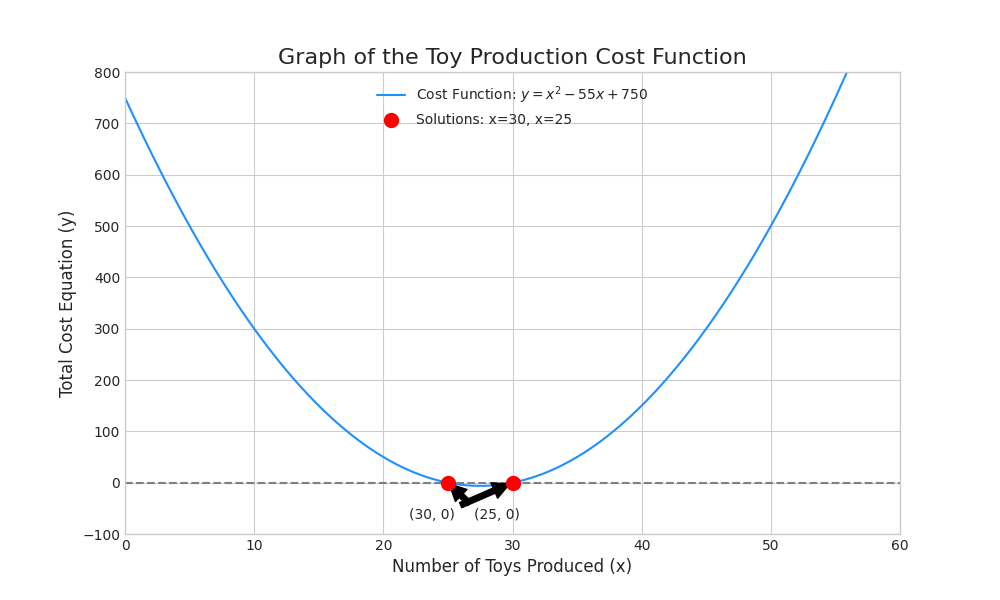
\includegraphics[width=0.75\columnwidth]{graph16.png}
        \caption{plot 9.4.24}
        \label{fig:placeholder}
    \end{figure}
\end{frame}
\end{document}